\documentclass[11pt]{article}


% -- Color scheme

% Color package
\usepackage{xcolor}

% Color scheme definitions

% Default
\definecolor{minimal-main}{HTML}{131313}
\definecolor{minimal-light}{HTML}{F2F2F2}
\definecolor{minimal-contrast}{HTML}{F3F2F5}

% Blue
%\definecolor{minimal-main}{HTML}{1E2839}
%\definecolor{minimal-light}{HTML}{EFF4F9}
%\definecolor{minimal-contrast}{HTML}{F3F2F5}

% Green
%\definecolor{minimal-main}{HTML}{083031}
%\definecolor{minimal-light}{HTML}{DEECE9}
%\definecolor{minimal-contrast}{HTML}{F3F2F5}

% Red
%\definecolor{minimal-main}{HTML}{361222}
%\definecolor{minimal-light}{HTML}{FFE8F2}
%\definecolor{minimal-contrast}{HTML}{F3F2F5}

% Additional color definitions
\definecolor{minimal-black}{HTML}{131313}
\definecolor{minimal-white}{HTML}{F3F2F5}
\definecolor{minimal-red}{HTML}{C43C2D}
\definecolor{minimal-blue}{HTML}{343454}
\definecolor{minimal-yellow}{HTML}{F1C40F}
\definecolor{minimal-green}{HTML}{2D6514}
\definecolor{minimal-beige}{HTML}{D7B6A5}

% Colorbox environments
\usepackage[most]{tcolorbox}


% -- Page layout

% Layout adjustments of page (a4 without margin)
\usepackage[paperheight=842pt, paperwidth=595pt, margin=0pt]{geometry}

% Remove paragraph indentation
\setlength{\parindent}{0pt}

% Interline spacing options
\newcommand{\largespace}{\\[2pt]}
\newcommand{\mediumspace}{\\[-3pt]}
\newcommand{\smallspace}{\\[-5pt]}

% In-box spacing around content
\newcommand{\inboxspacing}{.015\paperheight}

% Horizontal spacing of the boxes (must sum up to 1)
\newcommand{\sideboxwidth}{.35}
\newcommand{\mainboxwidth}{.65}

% Vertical spacing of the boxes (must sum up to 1)
\newcommand{\headboxheight}{.080}
\newcommand{\mainboxheight}{.910}
\newcommand{\footboxheight}{.010}

%   sideboxwidth           mainboxwidth
%  <------------> <---------------------------->
%  _____________________________________________
% |#############################################| ^
% |#############################################| |
% |################## HEADBOX ##################| | headboxheight
% |#############################################| |
% |#############################################| v
% |///////////////                              | ^
% |///////////////                              | |
% |///////////////                              | |
% |///////////////                              | |
% |////   ////////                              | |
% |//// S ////////              M               | |
% |//// I ////////              A               | |
% |//// D ////////              I               | |
% |//// E ////////              N               | | mainboxheight
% |//// B ////////              B               | |
% |//// O ////////              O               | |
% |//// X ////////              X               | |
% |////   ////////                              | |
% |///////////////                              | |
% |///////////////                              | |
% |///////////////                              | |
% |///////////////                              | v
% |#############################################| ^
% |################## FOOTBOX ##################| | footboxheight
% |#############################################| v


% -- Font settings

% Typesetting packages
\usepackage[letterspace=20]{microtype}
\usepackage[T1]{fontenc}

% Raleway font family
\usepackage[semibold]{raleway}
\renewcommand{\familydefault}{\sfdefault}

% Custom font commands
\newcommand{\header}[3]{\uppercase{\textbf{\fontsize{30}{100}{\lsstyle{#1 \hspace{3pt} #2 \hspace{3pt} #3}}}}}
\newcommand{\titlefont}[1]{\uppercase{\textbf{\Large{#1}}}}


% -- Additional packages

% Multirow tables
\usepackage{multirow}

% Settings for entire table columns (e.g \begin{tabular}{>{\footnotesize}rl})
\usepackage{array}

% Tikzpicture graphics
\usepackage{tikz}

% Clickable URLs
\usepackage{hyperref}
\urlstyle{same}


\begin{document}

\begin{tcbposter}[
    poster = {columns=1, rows=1, spacing=0pt},
    boxes = {sharp corners, halign=center, valign=center, boxrule=0pt}
]


% -- Headbox

\posterbox[
    colback=minimal-main,
    halign=center]
    {name=headbox,
    span=1,
    rowspan=\headboxheight}
{

    \color{white}

    \header{Maria}{Mezentseva}{}

    \vspace{-7px}
    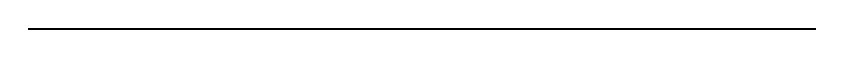
\begin{tikzpicture}
        \draw[fill=white] (-5.0, -0.01) rectangle (5.0, 0.01);
    \end{tikzpicture}
    \vspace{5px}

    \titlefont{But you can call me Maria Mezentseva}
}


% -- Sidebox

\posterbox[
    colback=minimal-light,
    valign=top,
    top=\inboxspacing,
    halign=right,
    right=\inboxspacing]
    {name=sidebar,
    below=headbox,
    column=1,
    span=\sideboxwidth,
    rowspan=\mainboxheight}
{

    \begin{tabular}{rl}

        \multicolumn{2}{@{}c@{}}{\scalebox{0.25}{\begin{tikzpicture}

    \fill[minimal-contrast] (-12.3, -16.7) rectangle (12.3, 16.7);
    
\begin{picture}(-12.3,-16.7)(0,0)
\put(-370,-467){
\includegraphics[width=700pt,height=950pt]{images/IMG_3544.png}}
\end{picture}
\end{tikzpicture}}} \\
        \mediumspace

        & \titlefont{Contact} \\
        \hline \mediumspace

        \multirow{4}{*}{\scalebox{0.075}{\input{icons/address.tex}}}
            & \textbf{Address} \\
                & Russian Federation \\
                & Dolgoprudniy \\
                & \smallspace

        \multirow{2}{*}{\scalebox{0.075}{\input{icons/phone.tex}}}
            & \textbf{Phone} \\
                & \href{https://www.youtube.com/watch?v=dQw4w9WgXcQ}{+42 42 4242-4242} \\
                & \smallspace

        \multirow{2}{*}{\scalebox{0.075}{\input{icons/email.tex}}}
            & \textbf{E-Mail} \\
                & \href{mailto:memezentseva@edu.hse.ru}{memezentseva@edu.hse.ru} \\
                & \largespace

        & \titlefont{Personal} \\
        \hline \mediumspace

        \multirow{2}{*}{\scalebox{0.075}{\input{icons/birthday.tex}}}
            & \textbf{Date of Birth} \\
                & 15/05/2001 \\
                & \smallspace

        \multirow{2}{*}{\scalebox{0.075}{\input{icons/nationality.tex}}}
            & \textbf{Nationality} \\
                & Russian \\
                & \largespace

        & \titlefont{Platforms} \\
        \hline \mediumspace

        \multirow{2}{*}{\scalebox{0.075}{\input{icons/github.tex}}}
            & \textbf{GitHub} \\
                & \href{https://github.com/morikarv}{morikarv} \\
                & \smallspace

        \multirow{2}{*}{\scalebox{0.075}{\input{icons/linkedin.tex}}}
            & \textbf{LinkedIn} \\
                & \href{https://www.linkedin.com/in/maria-mezentseva-b1153027b/}{Mezentseva Maria} \\
                & \largespace

        & \titlefont{Languages} \\
        \hline \mediumspace

        \multirow{2}{*}{\scalebox{0.075}{\input{flags/russia.tex}}}
            & \textbf{Russian} \\
                & Native \\
                & \smallspace

        \multirow{2}{*}{\scalebox{0.075}{\input{flags/britain.tex}}}
            & \textbf{English} \\
                & Fluent \\
                & \smallspace

        \multirow{2}{*}{\scalebox{0.075}{\input{flags/japan.tex}}}
            & \textbf{Japanese} \\
                & Basic

    \end{tabular}
}


% -- Mainbox

\posterbox[
    colback=white,
    valign=top,
    top=\inboxspacing,
    halign=left,
    left=\inboxspacing]
    {name=mainbox,
    column*=1,
    span=\mainboxwidth,
    below=headbox,
    rowspan=\mainboxheight}
{

    \begin{tabular}{>{\footnotesize}rl}

        & \titlefont{Education} \\
        \hline \mediumspace

        10/2022 - ongoing
            & \textbf{Higher School of Economics} \\
            & Bachelor's degree \\
            & Computer Science and Data Analysis \\
            & \mediumspace

        09/2019 - 11/2021
            & \textbf{Moscow Institute of Physics and Technology} \\
            & Bachelor's degree (not completed) \\
            & Applied physics and mathematics \\
            & \\
            & \largespace

        & \titlefont{Work Experience} \\
        \hline \mediumspace

        Since 05/2023
            & \textbf{LAMBDA (laboratory at HSE)} \\
            & Participating in project \\
            & Topic: ML and DL in anomalies detection \\
            & \\
            & \largespace

        & \titlefont{Technical Skills} \\
        \hline \mediumspace
        $\bullet$ $\bullet$ $\bullet$ $\bullet$ $\bullet$
            & \textbf{Python | Numpy, Pandas, SciPy, Seaborn, etc} \\
        $\bullet$ $\bullet$ $\bullet$ $\bullet$ $\circ$
            & \textbf{C++} \\
        $\bullet$ $\bullet$ $\bullet$ $\circ$ $\circ$
            & \textbf{Machine Learning} \\
        $\bullet$ $\circ$ $\circ$ $\circ$ $\circ$
            & \textbf{Deep Learning} \\
        $\bullet$ $\bullet$ $\bullet$ $\bullet$ $\circ$
            & \textbf{Matlab / Simulink} \\
        $\bullet$ $\bullet$ $\bullet$ $\bullet$ $\bullet$
            & \textbf{SQL} \\
        $\bullet$ $\bullet$ $\bullet$ $\bullet$ $\bullet$
            & \textbf{SolidWorks} \\
        $\bullet$ $\bullet$ $\bullet$ $\bullet$ $\bullet$
            & \textbf{FlowVision} \\
        $\bullet$ $\bullet$ $\bullet$ $\circ$ $\circ$
            & \textbf{git} \\
        $\bullet$ $\bullet$ $\bullet$ $\bullet$ $\bullet$
            & \textbf{Analysis and Acquiring of Experimental Data} \\
        $\bullet$ $\bullet$ $\bullet$ $\circ$ $\circ$
            & \textbf{Physics} \\
        $\bullet$ $\bullet$ $\bullet$ $\circ$ $\circ$
            & \textbf{Mathematical Methods in Data Analysis} \\
            & \\
            & \largespace
        & \titlefont{Soft Skills} \\
        \hline \mediumspace

        $\bullet$ $\bullet$ $\bullet$ $\bullet$ $\bullet$
            & \textbf{Teamwork | Gitlab, Notion, Github} \\
        $\bullet$ $\bullet$ $\bullet$ $\bullet$ $\circ$
            & \textbf{Speaking in front of the crowd} \\
            & \\
            & \largespace

        & \titlefont{Fields of Interest} \\
        \hline \mediumspace
        $\bullet$ $\bullet$ $\bullet$ $\bullet$ $\bullet$
            & \textbf{Astrophysics} \\
        $\bullet$ $\bullet$ $\bullet$ $\circ$ $\circ$
            & \textbf{Physics} \\
        $\bullet$ $\bullet$ $\bullet$ $\bullet$ $\bullet$
            & \textbf{Oceanology | Biology} \\
        $\bullet$ $\bullet$ $\bullet$ $\bullet$ $\bullet$
            & \textbf{Computer Vision} \\
            & \\
            & \largespace

        & \titlefont{Hobbies} \\
        \hline \mediumspace
            & Gaming \\
            & Board Games \\
            & Chess \\
            & \largespace 

    \end{tabular}
}


% -- Footbox

\posterbox[colback=minimal-main]
           {name=blankbox2,
           below=sidebar,
           column=1,
           span=1,
           rowspan=\footboxheight}{}

\end{tcbposter}

\end{document}